\chapter{Persistencia de visión (POV)}
\label{chap:persistenciaDeVision}

La persistencia de visión (\textsl{Persistence Of Vision}/\textbf{POV} en
Inglés) es un fenómeno óptico por el cual las imágenes que percibimos permanecen
durante un breve instante de tiempo en la retina (Persistencia retiniana).

Hasta hace poco se relacionaba con la percepción de movimiento. Posteriores
investigaciones en el campo de la neurofisiología de la percepción han
desmentido esta creencia, atribuyendo el fenómeno de percepcińo de movimiento a
complejos procesos neurológicos.

\label{def:radios}
Nuestro sistema se vale de este efecto óptico para construir imágenes
aparentemente completas, a partir de la suma de varias porciones de la misma
que se sucederán con suficiente rapidez para que permanezcan en nuestra
retina, creando así el efecto de la imagen completa. Un antiguo y sencillo
ejemplo de esto es el \textsl{taumatropo} (ver figura \ref{fig:taumatropo}), un
disco con una imagen en cada cara se hace girar rápidamente, creando un efecto
de superposición de ambas. En el caso de \textsl{CyclePOV} las ``porciones de
imagen'' van a ser varias lineas. Estas lineas se dispondrán de forma radial,
compartiendo uno de sus extremos. De esta forma, la sucesiva visualización de
estas ``porciones de imagen'' o ``lineas'' creará un efecto de imagen circular.
A estas lineas las vamos a denominar ``\textbf{radios}'' a lo largo del
documento.

\begin{figure}[!ht]
	\centering
	\begin{subfigure}[t]{0.4\textwidth}
		\centering
		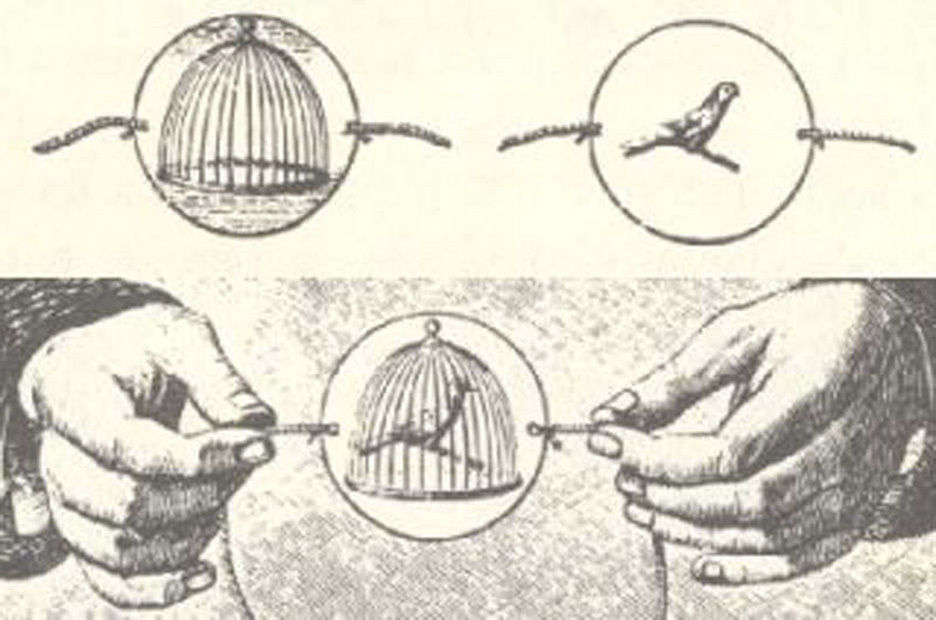
\includegraphics[width=\textwidth]{img/taumatropo}
		\caption{Taumatropo}
		\label{fig:taumatropo}
	\end{subfigure}
	\hspace{0.5cm}
	\begin{subfigure}[t]{0.4\textwidth}
		\centering
		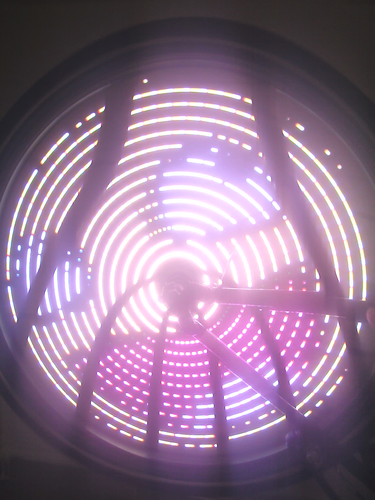
\includegraphics[width=\textwidth]{img/awesome}
		\caption{CyclePOV}
		\label{fig:awesome}
	\end{subfigure}
	\caption{Ejemplos de aplicaciones que aprovechan el POV}
\end{figure}
